\begin{figure}
    \centering
    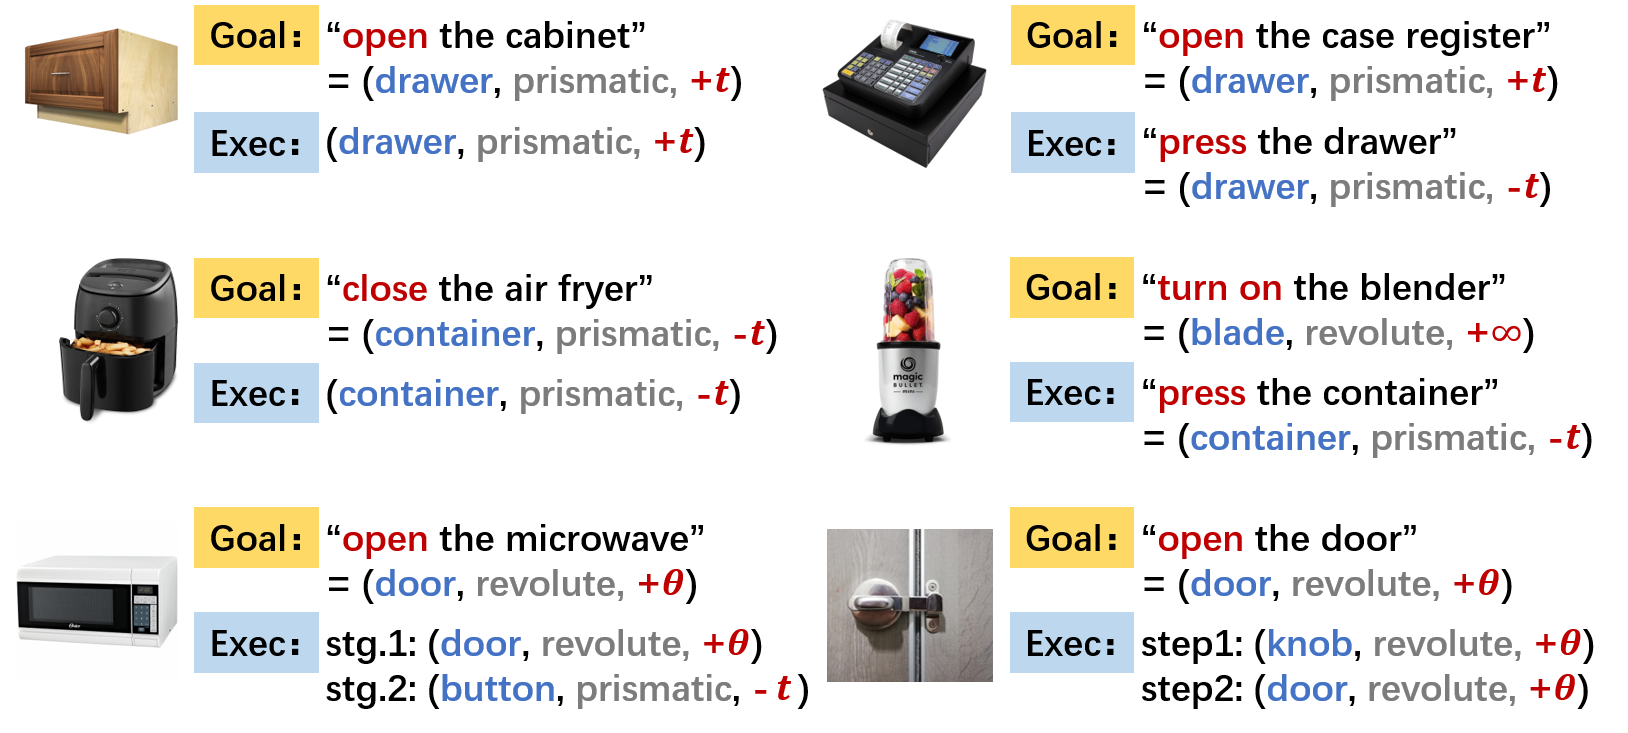
\includegraphics[width=\linewidth]{figures/tasks.png}
    \caption{\textbf{Objects, manipulation goals, and programmatic actions.}
    Each part-based action unit is represented as a 3-tuple of (part name, joint type, state change). Given the diverse structures and complex functionalities of the objects, the final action execution can be very different from the part state change directly implied by the input instruction.
    }
    \label{fig:tasks}
\end{figure}